% Nallino, Part II p. 242: the equation of the anomaly, redrawn from the print at the size of the print. The
% coordinates are those of a 400 dpi render of the figure (crop from x 114 pt, y 262 pt of the master page;
% y downward). ABD is the ecliptic about the Earth E, GHK the deferent about M (marked with a dot), E' the centre of
% the equant; the epicycle has its centre in H, the planet in T; ZHE', XxtHE and YTE are lines to the ecliptic,
% HT the radius of the epicycle, Tt (dotted) the perpendicular on EH. A stray dot to the right of K is not drawn.
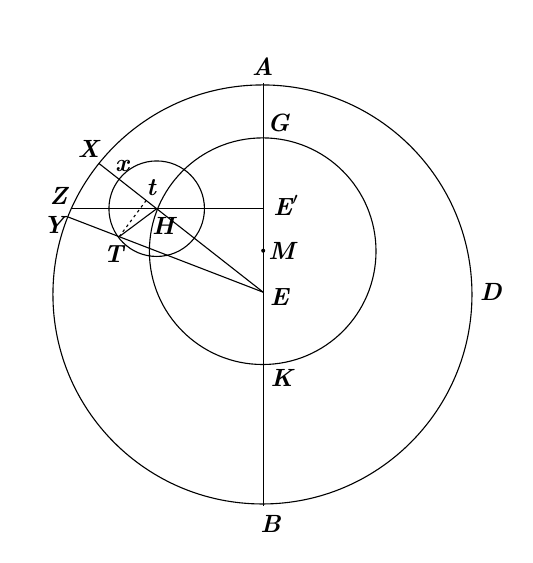
\begin{tikzpicture}[x=0.0635mm,y=-0.0635mm,line width=0.4pt,every node/.style={font=\bfseries\itshape\small,inner sep=1pt}]
\path (0,-22);
\coordinate (Ep) at (471,340);
\coordinate (M) at (471,424);
\coordinate (E) at (471,507);
\coordinate (H) at (258,340);
\coordinate (T) at (183,396);
\coordinate (t) at (237,323.5);
\coordinate (Z) at (87.2,340);
\coordinate (X) at (142.5,249.5);
\coordinate (Y) at (80.3,356.4);
\draw (469.5,511.5) circle[radius=419];
\draw (470,425) circle[radius=226.6];
\draw (H) circle[radius=95.5];
\draw (471,89) -- (471,935);
\draw (Z) -- (Ep);
\draw (X) -- (E);
\draw (Y) -- (E);
\draw (H) -- (T);
\draw[dash pattern=on 1pt off 1.2pt] (T) -- (t);
\fill (M) circle[radius=4];
\node at (470,56.5) {A};
\node at (501.5,169.5) {G};
\node at (121.5,220) {X};
\node at (189,255) {x};
\node at (247,298) {t};
\node at (61.5,315.5) {Z};
\node at (510,333) {E\rlap{$'$}};
\node at (52.5,373.5) {Y};
\node at (271,374) {H};
\node at (508,425) {M};
\node at (171.5,431) {T};
\node at (503,516) {E};
\node at (926,506.5) {D};
\node at (508,678.5) {K};
\node at (485.5,970.5) {B};
\end{tikzpicture}
